\chapter{Anwendungen von GANs}

\noindent Wie in den vorherigen Kapiteln gezeigt, sind GANs und seine Vielzahl an Varianten, in der Lage, eine Vielzahl von unterschiedlichen Aufgaben zu erfüllen, wobei die Arbeit mit visuellen und auditiven Inhalten aufgrund ihrer abstrakten Natur besonders hervorsticht. Im Folgenden werden die Möglichkeiten der Technologie in Form von drei konkreten visuellen Einsatzzwecken näher untersucht. \\

\section{Bildsynthese}

\noindent Einer der prominentesten und eindrucksvollsten Einsatzzwecke ist die Bildsynthese. Hierbei wird ein GAN trainiert, um Bilder zu generieren, die von einem menschlichen Auge nicht von echten Bildern unterschieden werden können. Häufig wird eine Conditional GAN verwendet, damit der Anwender die Eigenschaften des generierten Bildes genau bestimmen kann. Einige Produkte und Technologien, welche von GANs für die Bildsynthese Gebrauch machen, sind bereits heute über das Internet verfügbar, zum Beispiel Artbreeder. \\

\noindent Artbreeder, ehemals GANbreeder, ist eine Webseite, welche es dem Anwender ermöglicht, Bilder zu generieren, indem er die Eigenschaften von mehreren Bildern kombiniert. Die Webseite verwendet hierfür BigGAN, ein großes Modell, welches auf einem Datensatz von 150 Gigabyte an gelabelten Daten trainiert wurde. Dabei erlaubt Artbreeder nicht nur die Kombination bestimmter Motive, sondern erlaubt auch das freie Modifizieren bestimmter Faktoren. Bild \ref{fig:artbreeder} zeigt beispielsweise das stilisierte Bild einer Frau, welches durch Zugabe des Hundeparameters modifiziert wurde. So lassen sich abstrakte Konzepte realisieren, wie das Darstellen des Gegenteils eines Objekts. 

\newpage

\begin{figure}[H]
    \centering
    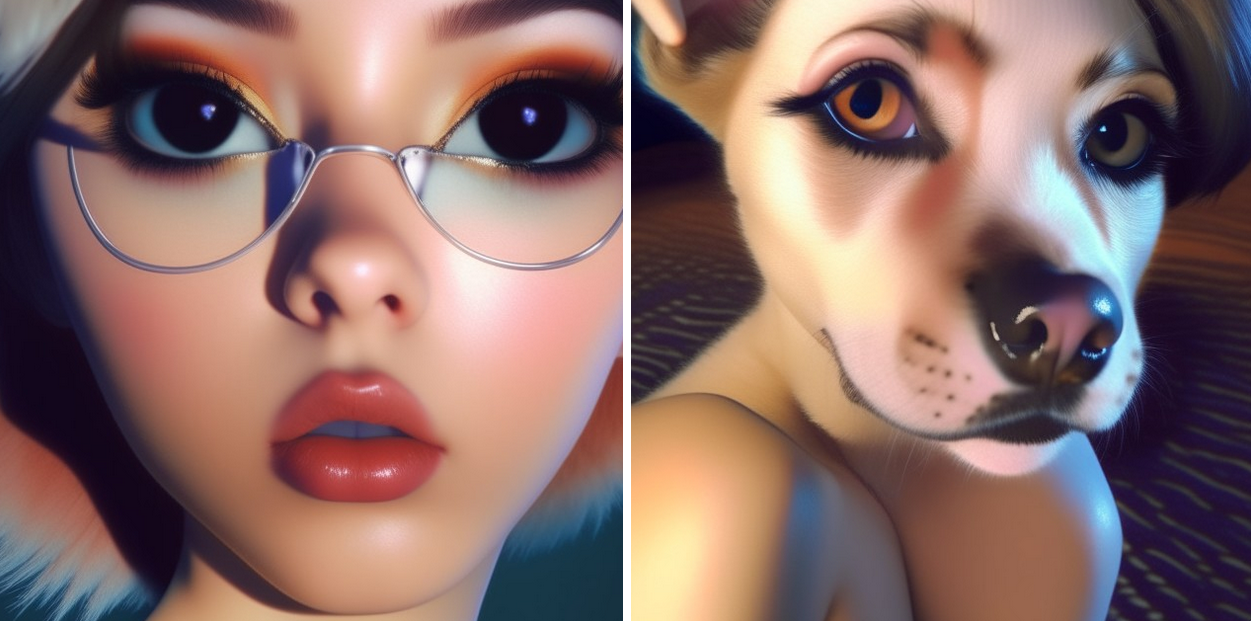
\includegraphics[width=0.8\textwidth]{Artbreeder}
    \caption{Demonstration von Artbreeder und Modifikation des Originals(links) durch Erhöhung des „Hundefaktors“} \quelle\url{https://www.artbreeder.com}
\label{fig:artbreeder}
\end{figure}


    
\noindent  Woran Artbreeder häufig scheitert, ist die Darstellung realistischer menschlicher Gesichter, welche häufig unnatürlich und seltsam wirken können.

\begin{wrapfigure}[18]{l}{0.50\textwidth}
    \centering
    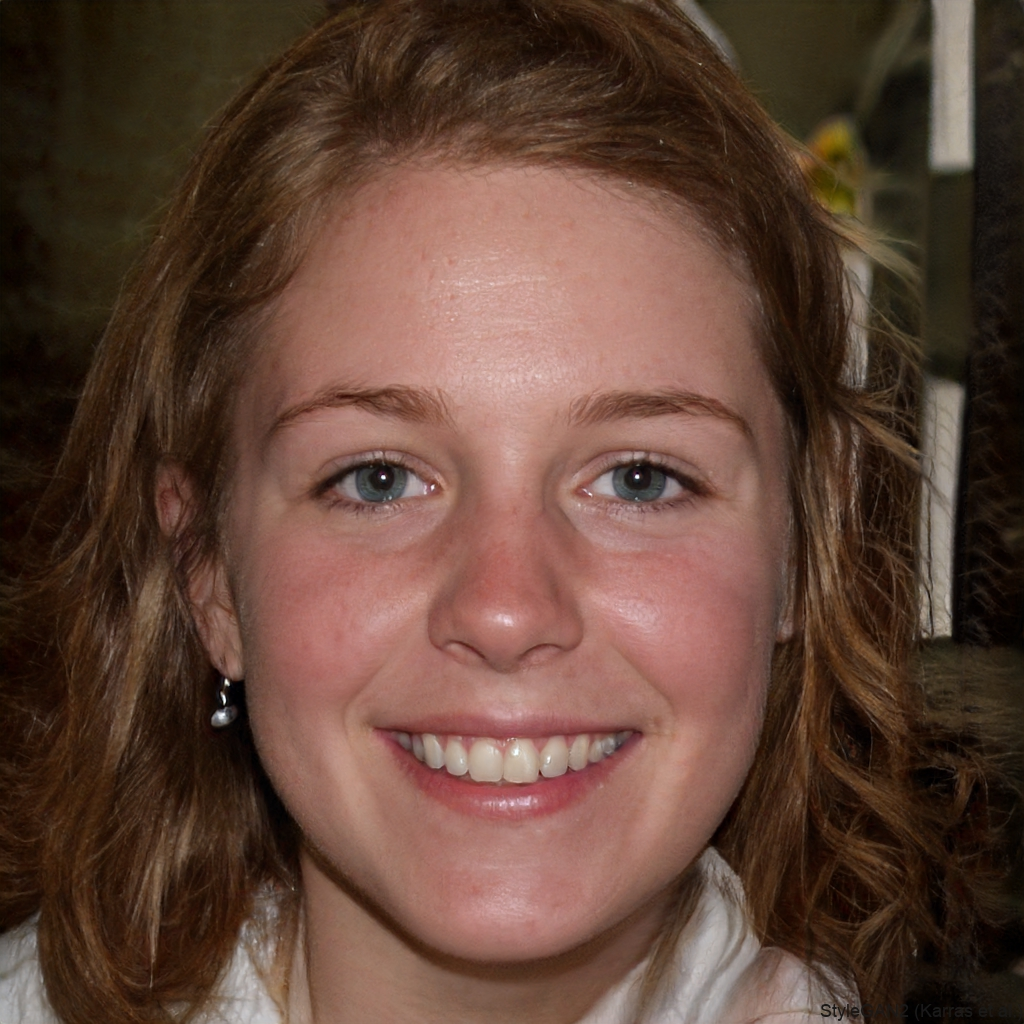
\includegraphics[width=0.50\textwidth]{this-person-does-not-exist}
    \caption{KI-genertiertes Gesicht} \quelle\url{https://thispersondoesnotexist.com/}
    \label{fig:tpdne}
    \end{wrapfigure}

\hfill
\break
Hier kommt StyleGAN ins Spiel. StyleGAN ist ein GAN, welches von Nvidia entwickelt wurde und sich auf die Generierung von Gesichtern spezialisiert hat. StyleGAN ist in der Lage, hochrealistische Bilder menschlicher Gesichter zu generieren, welche mit dem bloßen Auge kaum von echten menschlichen Gesichtern unterschieden werden können. Dies gilt besonders für StyleGAN 2, eine überarbeitete Version, die häufig auftretenden Artefakte reduziert und die generelle Bildqualität steigert. Ein bekannter und für jeden zugänglicher Beispiel für StyleGAN 2 ist „This Person does not exist“(siehe Bild \ref{fig:tpdne}), eine Webseite die bei Aufruf mithilfe dieses Netzes eine fotorealistisches Bild eines menschlichen Gesichts generiert.

\newpage
